%Empieza configuracion de capitulo

\setstretch{1.0}
\titleformat{\chapter}[block]{\Large\bfseries}{CHAPTER 
\Huge\thechapter\vspace{25 pt}}{0 pt}{\\\fontsize{26}{36}\selectfont}
\titlespacing{\chapter}{0 pt}{30 pt}{50 pt}[0 pt]
\titleformat{\section}{\Large\bfseries}{\thesection}{0 pt}{\hspace{30 pt}}
\titleformat{\subsection}{\large\bfseries}{\thesubsection}{0 pt}{\hspace{30 pt}}
\pagestyle{fancy}
\fancyhead[LO,LE]{\footnotesize\textit{\leftmark}}
\fancyhead[RO,RE]{\thepage}
\fancyfoot[CO,CE]{}
%Termina configuracion de capitulo

\chapter{Introduction} %Cambia Introducci'on al nombre de tu capitulo
\setstretch{1.5} %Regresa el interlineado a 1.5

\normalsize

This work Will present a detailed study of how could a network of embedded
systems collaborate among each others to solve parallel problems. After reading
this project you will understand how this can be done , what are their
limitations and recommendations if you would like to implement this as part of 
your current projects. 

\section{Background}
\vspace{30 pt}
\noindent

Our story begins decades ago. The Computers was finally at the homes and many
people wonder what was going to be next revolution. There was expectations that
in close future the Computers was going to be everywhere: in our houses , in
our cars teaching to the children and controlling the traffic. Well that was
the dream that seems more like a science fiction story. But as we know that
dream has came true in many ways.

All this has been possible due to the evolution of computing technology over
these years. Computer technology has made incredible progress in the roughly 60
years since the first general-purpose electronic computer was created. Today,
less than 500 dollars  will purchase a personal computer that has more
performance, more main memory, and more disk storage than a computer bought in
1985 for 1 million dollars. This rapid improvement has come both from advances
in the technology used to build computers and from innovation in computer
design.

The 1980s saw the rise of the desktop computer based on microprocessors, in the
form of both personal computers and workstations. The 1990s saw the emergence
of the Internet and the World Wide Web, the first successful handheld computing
devices, and the emergence of high-performance digital consumer electronics.
The extraordinary popularity of cell phones has been obvious since 2000, with
rapid improvements in functions and sales that far exceed those of the PC.
These more recent applications use embedded computers.

But lets stop a bit here. A new world came to our vocabulary at those days:
embedded. What is an embedded system? An embedded system is a special-purpose
system in which the computer is completely encapsulated by the device it
controls. Unlike a general-purpose computer, such as a personal computer, an
embedded system performs pre-defined tasks, usually with very specific
requirements. Examples of these was the first microwaves, the first cellphones
and GPS systems. All those electronic gadgets that started to emerge 10 years
ago.

As we know society loved these new devices and asked for more. Less cost, 
smaller devices, better power consumption and the capability to make much more
complex tasks. This was a clear path to follow until a new requirement came up:
Connectivity. The market started to ask for embedded systems with the capability
not only to measure but also with the capability to be fully connected to the
internet all the time. One could start to ask why. Why would I want to have an
embedded system connected to the internet all the time?. Can you imagine now
your TV, smart phone or tablet not connected to the Internet? This is the
technology that old science fiction novels imagine years ago, the internet of
things.

The Internet of Things (Iot) is defined as the interconnection via the Internet
of computing devices embedded in everyday objects, enabling them to send and
receive data. As you can see the differences with traditional embedded systems
are the internet connectivity and less power consumption

But the entire picture of an IoT solution is quite bigger. A full solution has 
the following parts:

\begin{itemize} 

\item The Thing (computing devices):  in the Internet of
Things, can be a person with a heart monitor implant, a farm animal with a bio
chip transponder, an automobile that has built-in sensors to alert the driver
when tire pressure is low or any other natural or man-made object that can be
assigned an IPA address and provided with the ability to transfer data over a
network 

\item Network Connection: Network Connections provides connectivity
between your computing devices  and the Internet, a network, or another compute
device 

\item Cloud computing Data centers for storage and Big Data analysis: The data
by itself is not useful to the end user. An alarm or recommendation is all that
the end user will matter. After the data is sent and stored into the Cloud
Computing Data Centers is necessary to run Big Data solutions that present
meaning full information to the users.  

\item Presentation Devices: At the end of the day, what do we do with all that
information we have collected?; one obvious thing is to display the information
via a dashboard. Dashboards have to be hosted on some kind of display, we call
that the Presentation Device.  It could be a desktop computer running an 
application, a tablet or a smart phone accesing to a web page. It could
even be a purpose-built device like a retail kiosk, intelligent vending machine
or a control panel. The goal is to present the information comming from the big
data analysis.

\end{itemize}


Like many booming areas of technology, the internet of things
revolution is plagued by a lack of industry standards. Right now exist two main 
projects that are compiling to establish standards for the IoT communications: 

\begin{itemize}
\item Open Interconnect Consortium (OIC): OIC is an industry group whose stated 
mission is to develop standards and certification for devices involved in the 
Internet of Things based around CoAP. OIC was created in July 2014 by Intel, 
Broadcom, and Samsung Electronics.

\item AllJoyn : AllJoyn is an open, universal, secure and programmable software 
connectivity and services framework that enables companies and enterprises to 
create interoperable products that can discover, connect and interact directly 
with other AllJoyn-enabled products.
\end{itemize}

Despite the efforts to develop standard, certifications and frameworks for 
interconnection among IoT systems there is no effort to make self sustainable 
networks. All the current solution send all the data to Cloud Data centers to be 
analyzed. 



\section{Problem Definition}
\noindent

We have to understand that the rise of the internet of things is real. According 
to a study by the International Data Corporation (IDC), a market research 
analysis and advisory firm specialized in information technology estimate the 
number of IoT devices is approaching  200 billion. And the number of sensors 
(e.g., the accelerometer in your smart phone) that track, monitor, or feed data 
to those things is already more than 50 billion, with scientists talking about 
trillion-sensor networks within 10 years.

Of course, not all of those 200 billion things are actually wired and 
communicating on the Internet, but some 20 billion are. And, by 2020, this 
number will grow by 50\% to 30 billion connected devices.

But the rise of the internet of things means the rise of data. The impact of the 
IoT is already visible in the digital universe. Data just from embedded systems 
(the sensors and systems that monitor the physical universe) already accounts 
for 2\% of the digital universe. By 2020 that will rise to 10\%.

There is one final way to look at : the load they will put on the IoT in terms 
of management. Computers don't just have to manage megabytes, they also have 
to manage the containers, or software-based digital files that the megabytes 
come in. Some containers are big, like a digital camera image . But some are 
small. RFID tags and sensor containers may contain as few as 32 bytes. Because 
of this small signal size, the number of containers that must be managed from 
these embedded systems will dominate the digital universe in 2020. We’re 
talking 99\% of all files in the digital universe.

Besides that, the power consumption of these  IoT’s Cloud Data Centers is a key
part to considerate. If current trends continue, a petaflop system will require 
100 megawatts to manage the IoT data. 

The rise of IoT will lead to an explosion in the volume of data collected, 
transmitted and processed.This will require novel and optimized solutions. 
How can we make the IoT networks self sustainable? Make them solve their own compute problems 
without the need to send millions of data to the HPC data centers . 

Imagine the current 200 billion IoT devices sending data to the cloud data 
centers at the same time. Adding more systems to the data center will increase 
the power consumption to the data center as well as the costs

\section{General Objective}
\noindent

The main objective is to present a methodology to crate a self sustainable
network of ultra-low-voltage microprocessors platforms. It means the embedded 
devices interconnected could process their own workload without the need of an 
external compute system

The purpose of this methodology is to give an experienced IoT  developer 
enough information to replicate the study. At the same time it offers the theoretical 
underpinning for understanding which method, set of methods, or so-called best 
practices can be applied an specific case


\section{Hypothesis}
\noindent

Nowadays most of the computer systems we use are distributed systems. These
systems are reliable, robust and fault tolerant. Thanks to this we are able to
have amazing technology (e-mails/video-streaming/media-chats). All these
technology has enforce the develop of better distributed systems

We already have all this technology for mobile systems that communicate with
data centers. This work will try to prove that is possible to adapt current
distributed systems technology to the embedded and IoT world. We will try to
prove this measuring the energy efficiency of a cluster of less than a dozed 
embedded systems. 

In computing, performance per watt is a measure of the energy efficiency of a
particular computer architecture or computer hardware. Literally, it measures
the rate of computation that can be delivered by a computer for every watt of
power consumed. 



\begin{equation}
    \dfrac {Performance}{Watts} = Energy
\end{equation}

Giving this the hypothesis we are trying to find to prove is that the energy
efficiency an embedded cluster will have is the 
figure~\ref{fig:1.2} on page~\pageref{fig:1.2}.


\begin{figure}[H]
\centering
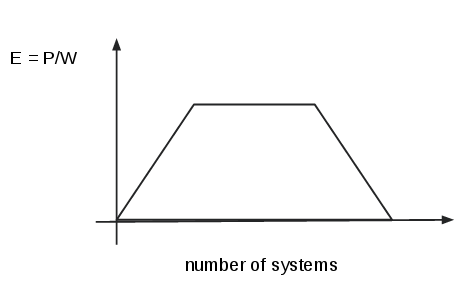
\includegraphics[width=0.75\textwidth]{images/graph_1.png}
\caption{Hypothesis of energy efficiency behavior in embedded cluster}
\label{fig:1.2}
\end{figure}

The way we are going to test this hypothesis requires the following parts:


\begin{itemize}
\item Chose the right embedded platform 
\item Chose the right Distributed System communication and compute protocol
\item Chose the right Operating System for the system (HW and communication protocol) 
\item Crate embedded clusters to measure energy efficiency
\item Improve communication protocol for embedded and IoT systems
\item Implement solution on real application ( greenhouse )
\end{itemize}

\section{Methodology}
\noindent

As described on the previous section the way we are trying to achieve this
research is as follows: 


\begin{itemize}
\item Chose the right embedded platform: There are dozens of embedded and IoT
    platforms, this is why is necessary to make a deep analysis and choose the
    best platform that feed our needs. Is important to mention that in a real
    application like a greenhouse the systems have an heterogeneous architecture.
\item Chose the right Distributed System communication and compute protocol.
    There are different kinds of distributed compute protocols. Part of this
    investigation is to detect the most reliable and suitable for our needs.
\item Chose the right Operating System for the system (HW and communication
    protocol). Once we have selected the appropriate embedded platforms, another 
    variable in this investigation is the number of Operating
    Systems. Either if is a micro kernel or a monolithic kernel architecture
    there are more than a dozen of chooses for the current embedded platforms
    exist on the market (the only requirement is that they have a microprocessor
    instead of a agriculturally)
\item Crate embedded clusters to measure energy efficiency. Once we have find
    the best configuration ( HW + OS + Communication Protocol ) and test this set
    up has the higher energy efficiency, we can start to create a cluster of
    embedded systems. The growth of Th cluster will be by 2 ( 2,4,6,8,10..) ;
    measuring at the same time the energy efficiency of the system.
\item Improve distributed technology for embedded and IoT systems. We will be
    focus on find improvements on the distributed technology (compute
    protocol, Operating System, Power and Performance) in order to make it part
    of world wide standards.
\item Implement solution on real application ( greenhouse ). In order to test
    or hypothesis in a real application we will implement it on a real
    greenhouse. Proving that the solution give an embedded system the power of
    reliability and availability without the need of external and expensive servers 
\end{itemize}


\clearpage
